\chapter{Bandera : génération de modèles à partir de code source Java}

Bandera est un logiciel permettant d'analyser un projet Java et d'en
extraire un modèle utilisable par un vérificateur de code. Il a été
développé suite à la collaboration de chercheurs de l'Université
d'Hawaï et de l'Université d'État du Kansas.

Ce logiciel n'est plus maintenu depuis 2005, néanmoins il peut être
intéressant de voir les décisions prises par ses développeurs pour
réaliser ce programme, car notre projet est en essence très similaire.

Nous allons donc étudier son fonctionnement, qui est détaillé dans
l'article~\cite{bandera1}.

\section{Postulat de base}

Les développeurs de Bandera partent d'un constat : des programmes de
vérification de modèle existent déjà, et permettent de comparer un
modèle représentant un programme à un modèle de
référence. Malheureusement, créer ce modèle à la main est un travail
long, fastidieux et sujet à des erreurs humaines. De plus, chaque
vérificateur attends le modèle dans son propre langage ou format de
fichier, ce qui signifie que pour vérifier un programme avec plusieurs
vérificateurs, il faut effectuer ce travail plusieurs fois.

\section{Transformation du code source}

Afin de transformer du code Java en un langage utilisable par des
vérificateurs, Bandera passe par un certain nombre de langages
intermédiaires. Il commence par traduire le programme en Jimple, un
langage utilisé par le framework Soot, et établit des correspondances
entre le code Java et le code Soot. Ceci permet au logiciel de
retrouver le n\oe{}ud Java correspondant à n'importe quel n\oe{}ud
dans Jimple.

L'arrière-plan (\textit{backend}) de Bandera s'occupe de traduire le
code Java en \gls{bir}, un langage bas niveau qui abstrait les
concepts communs à de nombreux logiciels de vérification de modèle. Le
but ce ce langage intermédiaire est de pouvoir ensuite exporter le
\gls{bir} dans différents langages spécialisés pouvant être utilisés
par les vérificateurs de modèles.

Ce fonctionnement est schématisé dans la figure~\ref{fig:bir_jimple}.

\begin{figure}[ht]
  \centering
  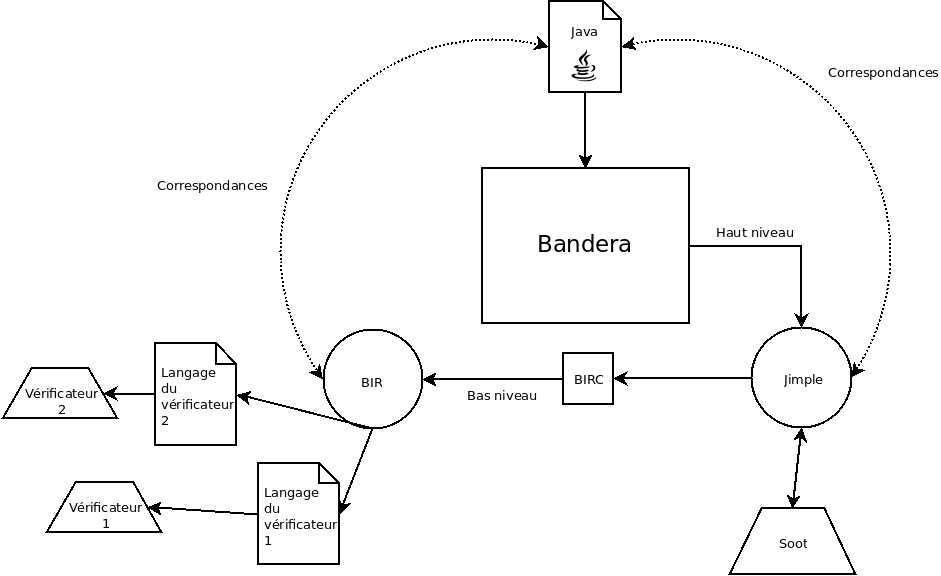
\includegraphics[scale=0.5]{images/bandera_bir_jimple.png}
  \caption{\label{fig:bir_jimple} Transformation du code source en
    langages intermédiaires}
\end{figure}


\section{Découpage (\textit{slicing}) du programme}

Dans le but de ne garder que les instructions intéressantes, Bandera
effectue un découpage des instructions. Pour un programme $P$, des
opérations $s_i$ sont extraites et regroupées dans $C$.

$$C = \{s_1, s_2, \ldots, s_k\}$$

Le découpage du programme va réduire $P$ afin de ne laisser que les
instructions nécessaires au bon fonctionnement des opérations
contenues dans $C$, et supprimer les autres.

Bandera se sert de cette méthode pour vérifier qu'un programme $P$
adhère à une spécification $\Phi$. Le logiciel supprime les
instructions de $P$ qui n'influent pas la satisfaction de $\Phi$. Si
$\Phi$ est juste pour la version réduite de $P$, alors $\Phi$ est
juste pour la version complète de $P$.

Découper un programme permet aussi de simplifier le travail du
vérificateur de modèle en réduisant le nombre d'instructions à
vérifier.